% Author: Seongjin Lee 
% Hanyang University, Seoul, Korea 
% esos.hanyang.ac.kr 
% 2016-09-01
% note: some slides are adopted from  \url{www.cs.stevens.edu/~jschauma/631A/}

\documentclass[newPxFont,sthlmFooter]{beamer}
\usepackage{kotex}
\usetheme{sthlm}
\hypersetup{pdfauthor={Seongjin Lee (insight@hanyang.ac.kr)},
            pdfsubject={Lecture Note: System Programming},
            pdfkeywords={Lecture Note, System Programming, class, undergraduate},
            pdfmoddate={D: \pdfdate},
            pdfcreator={Seongjin Lee}}

%\setbeamertemplate{footline}[text line]{%
%    \parbox{\linewidth}{\vspace*{-8pt} \insertsectionhead  \hfill\insertshortauthor\hfill\insertpagenumber}}
%\setbeamertemplate{navigation symbols}{}



\title{System Programming}
\subtitle{Week 1: Introduction to System Programming}
\author[SJL]{Seongjin Lee}
\institute{\href{mailto:insight@hanyang.ac.kr}{insight@hanyang.ac.kr}\\\url{http://esos.hanyang.ac.kr}\\Esos Lab. Hanyang University}
\date{2016-09-07} 

\begin{document}



\frame[plain]{\titlepage} 

\frame{\frametitle{Table of contents}\tableofcontents} 


%---------------------------------------------------------
\section{Nutshell} 

\begin{frame}[t]{}
\begin{figure}\centering
  \includegraphicscopyright[width=0.7\linewidth]
   {./figure/ken-dennis-pdp7.jpg}
   {Ken Thompson and Dennis Ritchie at PDP-11 in 1971 (Photo: \href{https://www.bell-labs.com/usr/dmr/www/kd14.jpg}{Courtesy of Bell Labs)}}
\end{figure}

\end{frame}






\begin{frame}[t]{What we are going to learn}
\begin{itemize}
 \item Familiarize with \textsc{Unix} 
 \item Experience systems programming
 \item Understand fundamental OS concepts
  \begin{itemize}
    \item Multi-user concepts
    \item Basic and advanced I/O
    \item Process
    \item Interprocess communication
  \end{itemize}
\end{itemize}
\end{frame}



\begin{frame}[t]{Why do we have to?}
\begin{itemize}
 \item \textsc{Unix} gives you insights on how other OS works
 \item You can only catch the tiger by going into the tiger's den
 \item It is the basis for most other programming and understanding of the system
 \item It in C helps you understand the general programming concepts
\end{itemize}
\end{frame}


\begin{frame}[t]{How are going to do?}
\lstinputlisting{./codes/welcome.c}

How to compile \\
\$ cc -Wall -g -o welcome welcome.c
\end{frame}

\begin{frame}[t,fragile]{Errors and Warnings}
\begin{lstlisting}
$ gcc -Wall -g -o welcome welcome.c
welcome.c:6:81: warning: implicit declaration of function 'getlogin' 
        is invalid in C99 [-Wimplicit-function-declaration]
        printf("Welcome to System Programming, %s!\n", getlogin())
                                                       ^
welcome.c:6:81: warning: format specifies type 'char *' but the 
        argument has type 'int' [-Wformat]
        printf("Welcome to System Programming, %s!\n", getlogin())
                                               ~~      ^~~~~~~~~~
                                               %d
welcome.c:6:92: error: expected ';' after expression
        printf("Welcome to System Programming, %s!\n", getlogin())
                                                                  ^
                                                                  ;
2 warnings and 1 error generated.
\end{lstlisting}


\end{frame}

\begin{frame}[t]{About this class}
Textbook
\begin{itemize}
	\item ``Advanced Programming in the UNIX Environment'', by
		W. Richard Stevens, Stephen A. Rago (3rd Edition)
\end{itemize}
\bigskip
Assistant
\begin{itemize}
	\item Yeonjin Noh (\href{mailto:nyg0813@gmail.com }{nyg0813@gmail.com})
	\item FTC \#804
\end{itemize}
\bigskip


\bigskip
Grading:
\vspace{-1em}
\begin{multicols}{2}
\begin{itemize}
	\item Attendance 5$\%$
	\item Assignments 30$\%$
	\item Quiz 5$\%$
	\item Midterm Exam 30$\%$
	\item Final Exam 30$\%$
	\item Level test on editors 
\end{itemize}
\end{multicols}
\end{frame}


\begin{frame}[t]{Syllabus}
\begin{columns}\small
\begin{column}{.48\linewidth}
\hangindent=1cm
Week 1 09-07 Introduction to system programming \& Shell Survival Kit
%\\•	Introduction, UNIX history, UNIX Programming Basics
%\\•	Working with Text Editor – Vi and Emacs (Level Test)
%\\•	Regular Expression

Week 2 09-14 (추석)

\hangindent=1cm
Week 3 09-21 Files IO \& ctag/etag
%\\•	File related operations
%\\•	Text editor with ctag/etag

\hangindent=1cm
Week 4 09-28 Files and Directories 
%\\•	On struct stat 
%\\•	Device special files
%\\•	Related operations

\hangindent=1cm
Week 5 10-05 Standard I/O Library
%\\•	Standard Input, output, and error
%\\•	Buffering
%\\•	Positioning a stream

\hangindent=1cm
Week 6 10-12 Process Environment
%\\•	Program Execution and Termination
%\\•	Memory Layout of a C program

Week 7 10-19 Process Control
%\\•	Process identifiers
%\\•	Process control operations

Week 8 10-26 (중간고사)
\end{column}

\begin{column}{.48\linewidth}
Week 9 11-02 Signals
%\\•	Concepts
%\\•	Interrupted system calls
%\\•	Related Functions

Week 10 11-09 Threads
%\\•	Thread concepts
%\\•	Creation and termination

Week 11 11-16 Thread Control
%\\•	Thread synchronization
%\\•	Locks

Week 12 11-23 Advanced I/O
%\\•	Non blocking I/O
%\\•	Memory mapped I/O

\hangindent=1cm
Week 13 11-30 Interprocess Communication I
%\\•	Pipes
%\\•	Message queues

\hangindent=1cm
Week 14 12-07 Interprocess Communication II
%\\•	Semaphores
%\\•	Shared memory

Week 15 12-14 Network IPC
%\\•	Vi and emacs (Level Test)
%\\•	Sockets
Week 16 12-21 (기말고사)
\end{column}
\end{columns}
\end{frame}



%---------------------------------------------------------
\section{History}
\begin{frame}[t]{The \textsc{Unix} History}
For more info : 
\url{http://www.unix.org/what_is_unix/history_timeline.html}
\bigskip
\begin{itemize}
	\item Originally developed in 1969 at Bell Labs by Ken Thompson
		and Dennis Ritchie.
	\item 1973, Rewritten in C. This made it portable and changed the history of OS
	\item 1974: Thompson, Joy, Haley and students at Berkeley develop
		the {\bf B}erkeley {\bf S}oftware {\bf D}istribution (BSD) of UNIX
	\item two main directions emerge: BSD and what was to become ``System V''
\end{itemize}
\end{frame}

\begin{frame}[t]{\textsc{Unix} History}
\begin{itemize}\small
	\item 1984 4.2BSD released (TCP/IP)
	\item 1986 4.3BSD released (NFS)
	\item 1991 Linus Torvalds starts working on the Linux kernel
	\item 1993 Settlement of USL vs. BSDi; NetBSD, then FreeBSD are created
	\item 1994 Single UNIX Specification introduced
	\item 1995 4.4BSD-Lite Release 2 (last CSRG release); OpenBSD
		forked off NetBSD
	\item 2000 Darwin created (derived from NeXT, FreeBSD, NetBSD)
	\item 2003 Xen; SELinux
	\item 2005 Hadoop; DTrace; ZFS; Solaris Containers
	\item 2006 AWS ("Cloud Computing" comes full circle)
	\item 2007 iOS; KVM appears in Linux
	\item 2008 Android; Solaris open sourced as OpenSolaris
\end{itemize}

list from \url{www.cs.stevens.edu/~jschauma/631A/}

\end{frame}



\begin{frame}[c]{History}
\centering
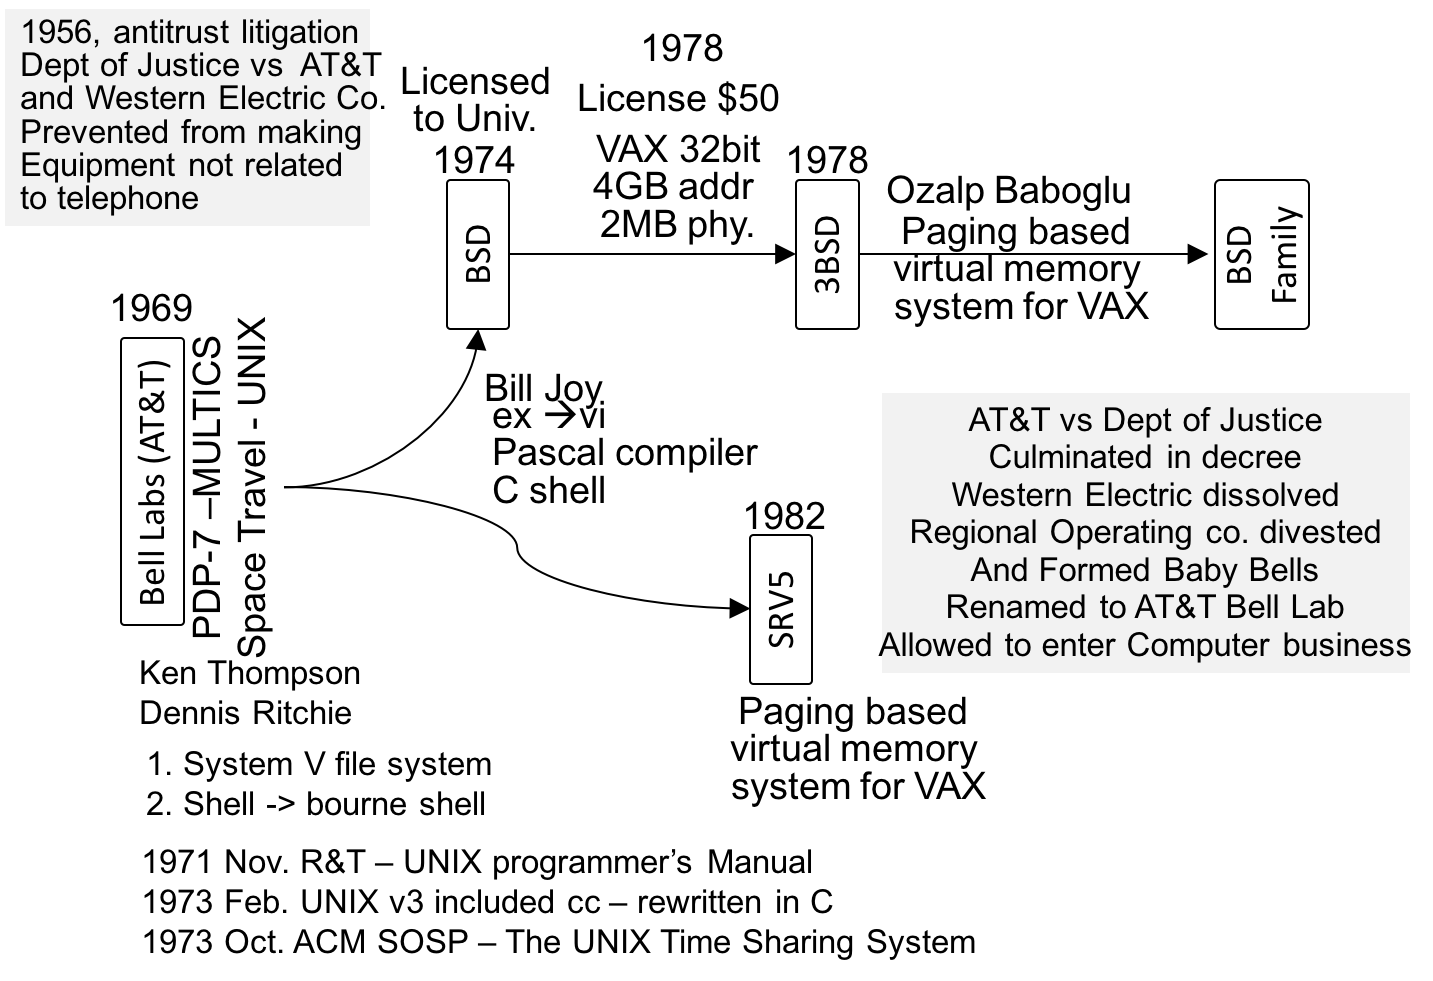
\includegraphics[width=0.9\textwidth]{./figure/history_1.png}
\end{frame}


\begin{frame}[c]{History}
\centering
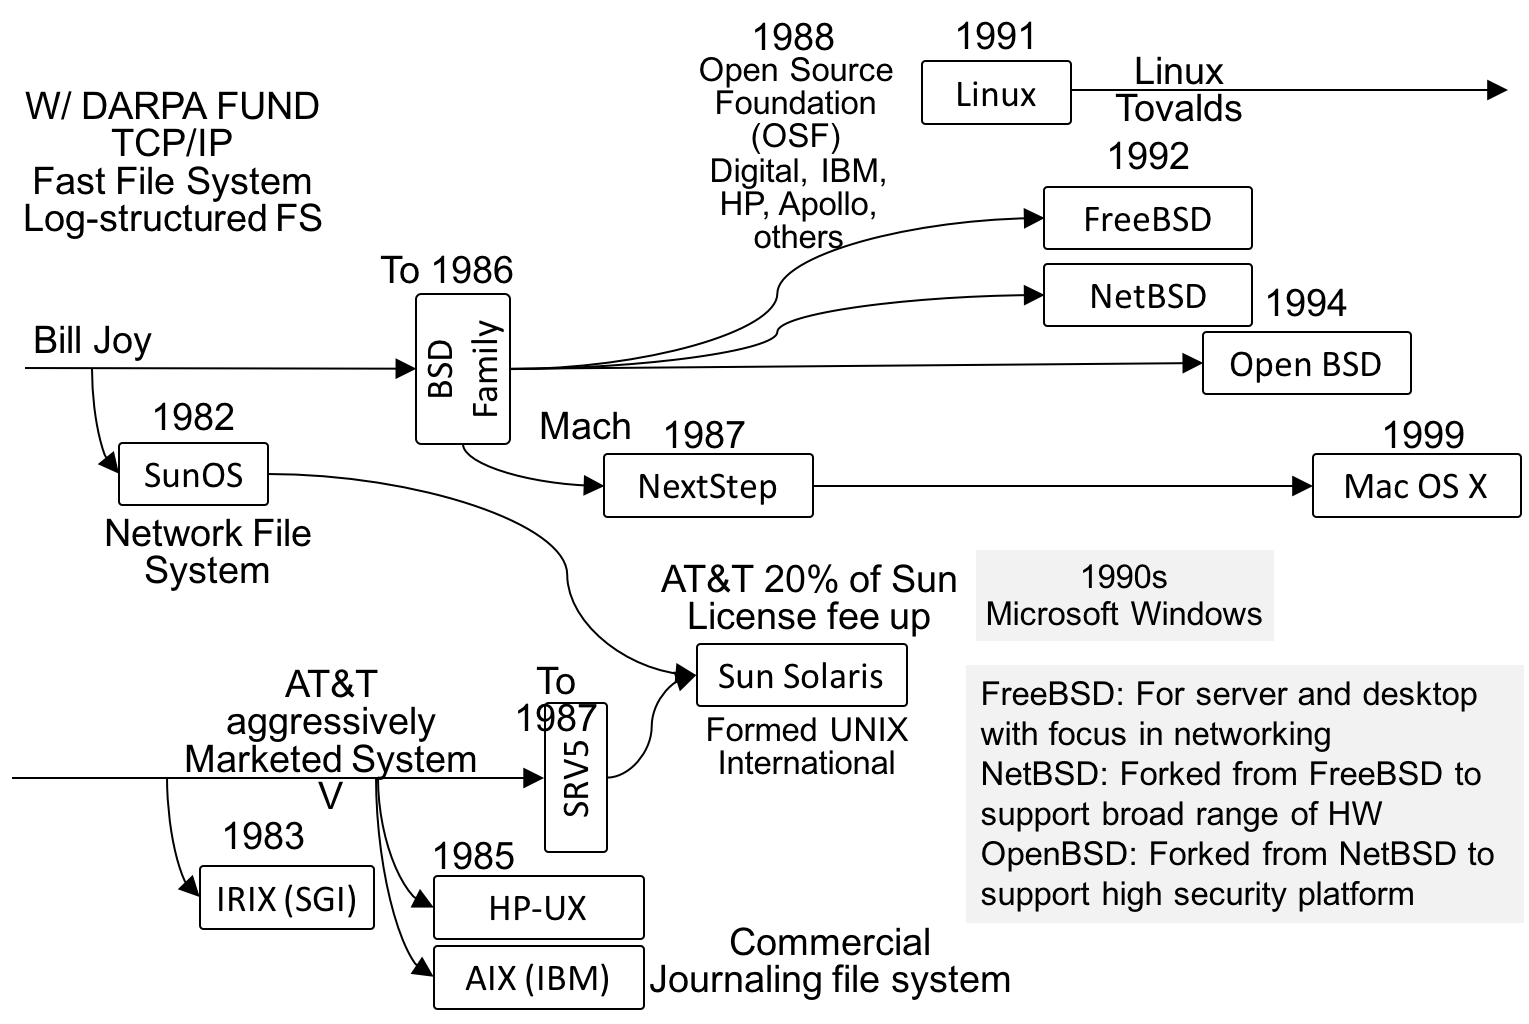
\includegraphics[width=0.9\textwidth]{./figure/history_2.png}
\end{frame}


\begin{frame}[t]{Some \textsc{Unix} Versions}
More UNIX (some generic, some trademark, some just unix-like):
\\
{
\fontsize{5pt}{6pt}\selectfont
\begin{tabular}{ c c c c c}
	1BSD & 2BSD & 3BSD & 4BSD & 4.4BSD Lite 1 \\
	4.4BSD Lite 2 & 386 BSD & A/UX & Acorn RISC iX & AIX \\
	AIX PS/2 & AIX/370 & AIX/6000 & AIX/ESA & AIX/RT \\
	AMiX & AOS Lite & AOS Reno & ArchBSD & ASV \\
	Atari Unix & BOS & BRL Unix & BSD Net/1 & BSD Net/2 \\
	BSD/386 & BSD/OS & CB Unix & Chorus & Chorus/MiX \\
	Coherent & CTIX & Darwin & Debian GNU/Hurd & DEC OSF/1 ACP \\
	Digital Unix & DragonFly BSD & Dynix & Dynix/ptx & ekkoBSD \\
	FreeBSD & GNU & GNU-Darwin & HPBSD & HP-UX \\
	HP-UX BLS & IBM AOS & IBM IX/370 & Interactive 386/ix & Interactive IS \\
	IRIX & Linux & Lites & LSX & Mac OS X \\
	Mac OS X Server & Mach & MERT & MicroBSD & Mini Unix \\
	Minix & Minix-VMD & MIPS OS & MirBSD & Mk Linux \\
	Monterey & more/BSD & mt Xinu & MVS/ESA OpenEdition & NetBSD \\
	NeXTSTEP & NonStop-UX & Open Desktop & Open UNIX & OpenBSD \\
	OpenServer & OPENSTEP & OS/390 OpenEdition & OS/390 Unix & OSF/1 \\
	PC/IX & Plan 9 & PWB & PWB/UNIX & QNX \\
	QNX RTOS & QNX/Neutrino & QUNIX & ReliantUnix & Rhapsody \\
	RISC iX & RT & SCO UNIX & SCO UnixWare & SCO Xenix \\
	SCO Xenix System V/386 & Security-Enhanced Linux & Sinix &
		Sinix ReliantUnix & Solaris \\
	SPIX & SunOS & Tru64 Unix & Trusted IRIX/B & Trusted Solaris \\
	Trusted Xenix & TS & UCLA Locus & UCLA Secure Unix & Ultrix \\
	Ultrix 32M & Ultrix-11 & Unicos & Unicos/mk & Unicox-max \\
	UNICS & UNIX 32V & UNIX Interactive & UNIX System III & UNIX System IV \\
	UNIX System V & UNIX System V Release 2 & UNIX System V Release 3 &
		UNIX System V Release 4 & UNIX System V/286 \\
	UNIX System V/386 & UNIX Time-Sharing System & UnixWare & UNSW & USG \\
	Venix & Wollogong & Xenix OS & Xinu & xMach \\
\end{tabular}
}
\bigskip

\hfill {\footnotesize adopted from \url{http://www.cs.stevens.edu/~jschauma/631A/}}
\end{frame}





%---------------------------------------------------------
\section{The \textsc{Unix} Basics}

\begin{frame}[t]{The \textsc{Unix} Basics: Architecture}
applications $>$ shell
\bigskip
~
\centering
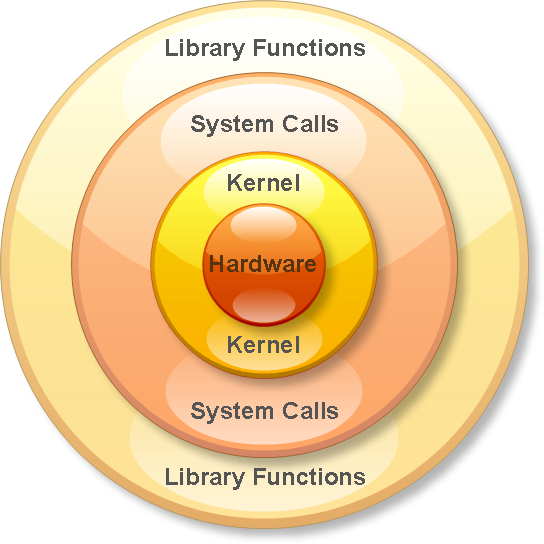
\includegraphics[height=0.85\textheight]{./figure/System-Call-and-Library-Function.png}
\end{frame}



\begin{frame}[t]{System Calls and Library Calls}
\begin{block}{System calls} 
They are entry points into kernel code where their functions are implemented.  Documented in section 2 of the manual (e.g. \texttt{write(2)} or \texttt{\$man 2 write}).
\end{block}
\bigskip

\begin{block}{Library Calls}
They are transfers to user code which performs the desired functions. Documented in section 3 of the manual (e.g. \texttt{printf(3)}).
\end{block}
\end{frame}


\begin{frame}[containsverbatim,t]{Error Handling: ANSI C}
\begin{itemize}
	\item	Important ANSI C Features:
		\begin{itemize}
			\item function prototypes
			\item generic pointers ({\tt void *})
			\item abstract data types (e.g. {\tt pid\_t}, {\tt size\_t})
		\end{itemize}
	\item	Error Handling:
		\begin{itemize}
			\item meaningful return values
			\item {\tt errno} variable
			\item look up constant error values via two functions:
		\end{itemize}
\end{itemize}

\begin{lstlisting}
#include <string.h>
char *strerror(int errnum) // returns pointer to message string
\end{lstlisting}

\bigskip

\begin{lstlisting}
#include <stdio.h>
void perror(const char *msg)
\end{lstlisting}

\end{frame}

\begin{frame}[t]{Principles}
\url{https://en.wikipedia.org/wiki/Unix_philosophy}
\bigskip
\begin{itemize}
\item Small is beautiful.
\item Make each program do one thing well.
\item Build a prototype as soon as possible.
\item Choose portability over efficiency.
\item Store data in flat text files.
\item Use software leverage to your advantage.
\item Use shell scripts to increase leverage and portability.
\item Avoid captive user interfaces.
\item Make every program a filter.
\end{itemize}
\end{frame}



%---------------------------------------------------------
\section{The Editors}
\subsection{Vim}

\begin{frame}[t]{}
\begin{figure}\centering
  \includegraphicscopyright[width=\linewidth]
   {./figure/vi_why.png}
   {\centering Image from \url{http://michael-prokop.at/computer/tools_vim_en.html}}
\end{figure}
\end{frame}

\begin{frame}[t]{What is Vi(m)}
\textbf{Vi} is a visual screen text editor developed by Bill Joy, who later becomes co-founder of Sun Micro Systems 
\begin{itemize}
\item It is visual version of \textbf{ex}, a Unix line editor
\item Vi is available on most Unix Systems
\item Works with a variety of terminals
\item Allows \textbf{ex} command from \textbf{vi}
\end{itemize}
\bigskip

\begin{center}
 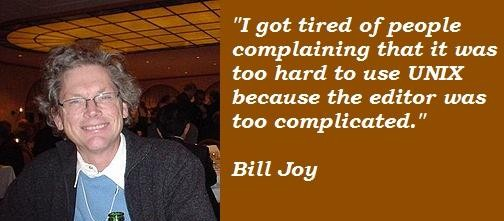
\includegraphics[width=0.7\linewidth]{./figure/bill_joy_quotes.jpg}
\end{center}
\end{frame}


\begin{frame}[t]{What is Vim}
\begin{columns}
\begin{column}{0.8\linewidth}
\textbf{VIM} is acronym for \textbf{Vi} i\textbf{M}proved, developed by Bram Moolenaar, a extended version of vi and some of enhancements include
\begin{itemize}
\item Completion, comparison, and merging of files
\item Split and tabbed windows
\item Command histories
\end{itemize}
\bigskip
All editing session before saving is done in buffer area
\begin{itemize}
\item Nothing is saved as hard data, until you save it
\end{itemize}
\end{column}
\begin{column}{0.2\linewidth}
  
\includegraphics[width=0.8\linewidth]{./figure/vim_logo.png}
\end{column}
\end{columns}
\end{frame}


\begin{frame}[t]{Modes of vi}
There are three mode in vi
\begin{itemize}
\item \textbf{Command Mode} – A default mode in vi
\begin{itemize}
\item Everything is command before you enter into other modes
\end{itemize}
\item \textbf{Input Mode} – What you type is what you see
\begin{itemize}
\item Anything typed in this mode is considered as data
\item Pressing [ESC] always leads to Command mode
\end{itemize}
\item \textbf{Last Line Mode} – Only can be accessed from Command mode
\begin{itemize}
\item Three ways to enter Last Line Mode – : (Colon) / (Back Slash) ? (Question Mark)
\end{itemize}
\end{itemize}
\begin{center}
 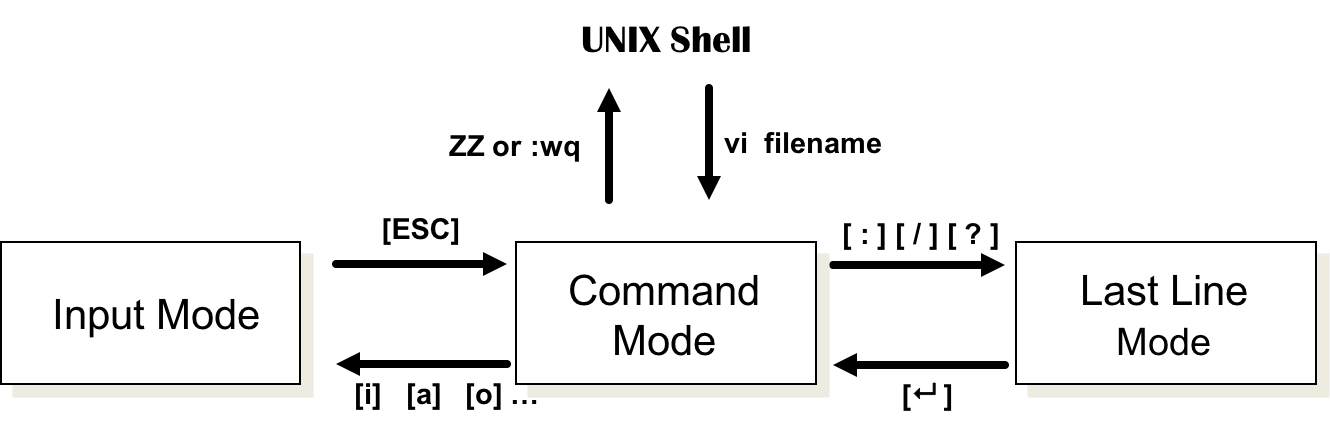
\includegraphics[width=0.8\linewidth]{./figure/vi_modes.png}
\end{center}
\end{frame}




\begin{frame}[t]{Moving Around}
VI uses four characters to move around, and each character is mapped to a direction

\begin{center}
 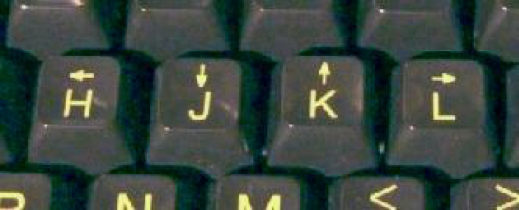
\includegraphics[width=0.7\linewidth]{./figure/vi_directions.png}
\end{center}

Moving by units of word, sentence, paragraph
\begin{itemize}
\item E.g., 3w moves to three words after the current cursor
\end{itemize}


\keystroke{w} next word \hfill \keystroke{b} previous word \hfill \keystroke{(} Beginning of sentence 

\bigskip
\keystroke{)} end of sentence \hfill \keystroke{\{} Beginning of paragraph \hfill \keystroke{\}} end of paragraph 
\end{frame}


\begin{frame}[t]{Deleting}
Deleting a character, words, sentence, line, and paragraph
\begin{itemize}
 \item \keystroke{x} erases a character
 \item Combination of direction commands with \keystroke{d} erases a word, sentence, and paragraph.
\begin{itemize}
\item E.g., \keystroke{dw} erases a word before the cursor
\end{itemize}
 \item \keystroke{dd} erases a line
 \item \keystroke{D} to delete rest of line
 \item \keystroke{X} to delete before the cursor
 \item \keystroke{Xp} to transpose
\end{itemize}

\end{frame}



\begin{frame}[t]{Searching and Replacing}
Searching in vi is done in last line mode
\begin{itemize}
\item \keystrokered{/} lets you search a character, word, and words
\begin{itemize}
\item E.g., \keystroke{/abc} moves the cursor to the location of the pattern
\end{itemize}
\item Search pattern in forward direction: \keystroke{n}, backward direction: keystroke{N}
\item Regular expressions can be also used in searching
\end{itemize}
\bigskip

\keystroke{r} replaces a character 
\begin{itemize}
\item Suppose the cursor is on \keystroke{b}, and by \keystrokered{r} \keystroke{p} we can change it to “preview”
\end{itemize}
\begin{center}
\keystroke{breview} $\rightarrow$ \keystrokered{preview}
\end{center}

\end{frame}


\begin{frame}[t]{Substitution}
\begin{center}
\textbf{Substituting in vi is done in last line mode}
\end{center}
\bigskip
Find i and substitute with X once
\vspace{0.5em}
\begin{center}
\begin{tabular}{ p{1cm} c p{3cm} c p{3cm}} 
\keystrokered{:s/i/X} & $\rightarrow$ & This is preview. How it is done & $\rightarrow$ & ThXs is preview. How it is done \\
\end{tabular}
\end{center}
\bigskip
Find i and substitute with X in the same line
\vspace{0.5em}
\begin{center}
\begin{tabular}{ p{1cm} c p{3cm} c p{3cm}} 
\keystrokered{:s/i/X/g} & $\rightarrow$ & This is preview. How it is done & $\rightarrow$ & ThXs is prevXew. How it is done \\
\end{tabular}
\end{center}
\bigskip
Find i and substitute with X in all the lines
\vspace{0.5em}
\begin{center}
\begin{tabular}{ p{1cm} c p{3cm} c p{3cm}} 
\keystrokered{:\%s/i/X/g} & $\rightarrow$ & This is preview. How it is done & $\rightarrow$ & ThXs is prevXew. How Xt Xs done \\
\end{tabular}
\end{center}
\end{frame}




\begin{frame}[t]{Undo and Redo}
Undo in vi is done by \keystroke{u} 
\begin{itemize}
\item Or to do in last line mode you could type in \keystroke{:undo}
\item \keystroke{U} undo all latest changes on one line
\end{itemize}
\bigskip

Redo in vi is done by \keystroke{CTRL}\keystroke{R} 
\begin{itemize}
\item Or to do in last line mode you could type in \keystroke{:redo}
\end{itemize}

\end{frame}



\begin{frame}[containsverbatim,t]{Simple Tutorial: From Start to quit}
This simple tutorial illustrates how to write, delete, copy, paste, replace, save, and quit. Start \texttt{vi} by \texttt{vi newfile.txt}  and type the following
\begin{beamercolorbox}[sep=1em,wd=\linewidth]{boxsthlmLightOrange}
\keystroke{i}~ This is how we write \keystroke{esc}~ \keystroke{o}~ and copy lines \keystroke{esc}~ \keystroke{k}~ \keystroke{y}~\keystroke{y}~ \keystroke{j}~ \keystroke{p}~ 
\keystroke{k}~ \keystroke{y}~ \keystroke{3}~ \keystroke{w}~ \keystroke{j}~ \keystroke{)}~ \keystroke{a}~ \keystroke{space bar}~ \keystroke{esc}~ \keystroke{p}~ \keystroke{o}~ ummm \keystroke{esc}~ \keystroke{b}~ \keystroke{x}~ \keystroke{r}~ 
E \keystroke{l}~ \keystroke{r}~ N \keystroke{l}~ \keystroke{r}~ D \keystroke{:}~ \keystroke{w}~ \keystroke{q}~ \keystroke{enter}~
\end{beamercolorbox}
\bigskip

This will produce following and goes back to command prompt

\begin{beamercolorbox}[wd=\linewidth]{boxsthlmLightPurple}
\begin{sthlmLatex}This is how we write 
and copy lines
This is how we write and copy lines
END\end{sthlmLatex}
\end{beamercolorbox}

\end{frame}



\begin{frame}[containsverbatim,t]{Simple Tutorial: From Start to quit}
\begin{beamercolorbox}[sep=1em,wd=\linewidth]{boxsthlmLightOrange}
\keystroke{i}~ This is how we write \keystroke{esc}~ \keystroke{o}~ and copy lines \keystroke{esc}~ \keystroke{k}~ \keystroke{y}~\keystroke{y}~ \keystroke{j}~ \keystroke{p}~ 
\keystroke{k}~ \keystroke{y}~ \keystroke{3}~ \keystroke{w}~ \keystroke{j}~ \keystroke{)}~ \keystroke{a}~ \keystroke{space bar}~ \keystroke{esc}~ \keystroke{p}~ \keystroke{o}~ ummm \keystroke{esc}~ \keystroke{b}~ \keystroke{x}~ \keystroke{r}~ 
E \keystroke{l}~ \keystroke{r}~ N \keystroke{l}~ \keystroke{r}~ D \keystroke{:}~ \keystroke{w}~ \keystroke{q}~ \keystroke{enter}~
\end{beamercolorbox}

The command in the tutorial

\begin{beamercolorbox}[sep=1em,wd=\linewidth]{boxsthlmLightPurple}
\keystroke{i} insert \hfill \keystroke{esc} back to command mode \hfill \keystroke{o} add new line after current line \hfill \keystroke{k} move cursor up \hfill \keystroke{yy} copy a line \hfill \keystroke{j} move cursor down \hfill \keystroke{p} paste after cursor point \hfill  \keystroke{y3w} copy three words \hfill \keystroke{)} move to end of sentence \hfill \keystroke{a} append \hfill \keystroke{b} move cursor to previous word \hfill \keystroke{x} erase a character \hfill \keystroke{r} replace a character \hfill \keystroke{l} move cursor right \hfill \keystroke{:wq} write to a file and quit 
\end{beamercolorbox}

\end{frame}



\begin{frame}[containsverbatim,t]{Learn by experience}

\lstinputlisting{./codes/learnbyexperience.txt}


Complete all tasks with minimum number of retyping, but with commands
\begin{itemize}
\item Substitute all j's to z and all z's to j
\item Copy lines 1, 3, 5, and 6, and make new paragraph with those lines
\item Delete three words ``requires extra pluck,'' and type in ``need lot of money'' in the place
\item Add ``caps'' at the end of all words with ``w'', e.g., wizards to ``wizardscaps''
\end{itemize}


\end{frame}



\begin{frame}[t]{References}
Graphical cheat sheet of Vi and VIM
\begin{itemize}
\item \url{http://www.viemu.com/a_vi_vim_graphical_cheat_sheet_tutorial.html}
\end{itemize}

Cursor movement Commands
\begin{itemize}
\item \url{http://www.kcomputing.com/vi.html}
\end{itemize}

List of Commands 
\begin{itemize}
\item \url{http://www.smashingmagazine.com/2010/05/03/vi-editor-linux-terminal-cheat-sheet-pdf/}
\end{itemize}

\bigskip\centering
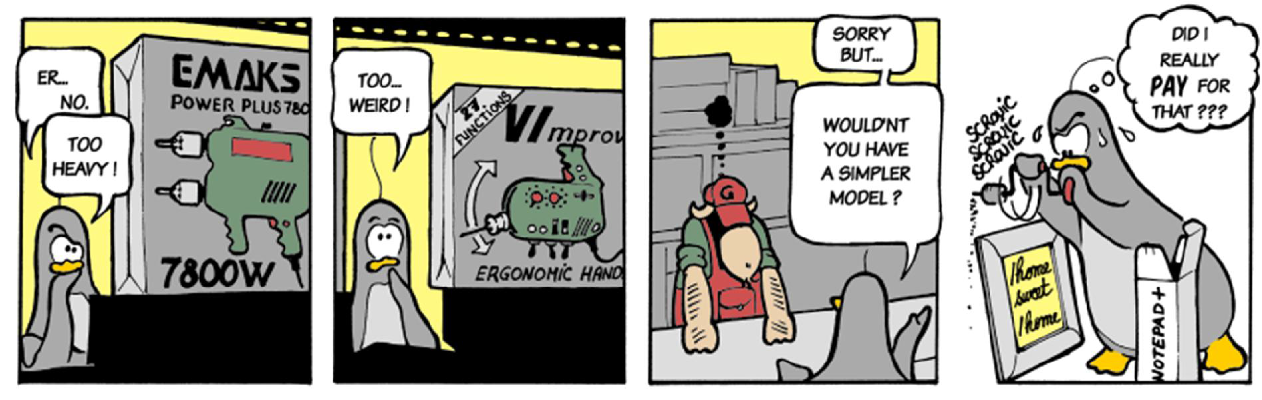
\includegraphics[width=0.9\textwidth]{./figure/vi_tools.png}
\end{frame}




%---------------------------------------------------------
\subsection{Emacs}

\begin{frame}[t]{}
\centering
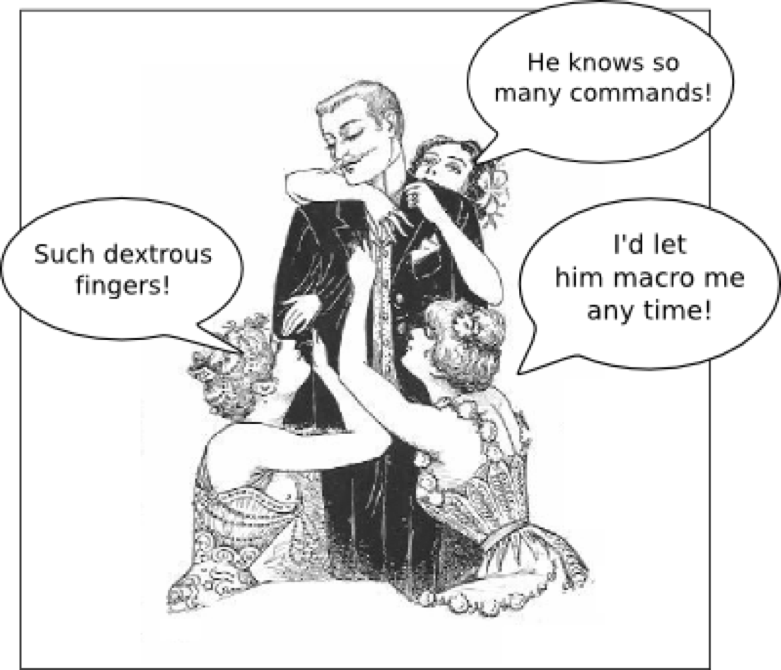
\includegraphics[width=0.9\textwidth]{./figure/emacs_dex.png}
\end{frame}


\begin{frame}[t]{What is Emacs}
\vspace{-1.5em}
\begin{columns}
\begin{column}{.7\linewidth}
Emacs (Editor MACroS) is the extensible, customizable, self-documenting, real-time display editor

\bigskip
Richard Stallman is the author of Emacs; the author of GCC and GDB

\bigskip
Runs on LISP engines + lots of LISP libraries
\end{column}
\begin{column}{.3\linewidth}
\begin{figure}\centering
  \includegraphicscopyright[width=\linewidth]
   {./figure/richard_stallman.png}
   {\href{https://regmedia.co.uk/2012/06/12/richard_stallman.jpg}{http://www.theregister.co.uk/}}
\end{figure}
\end{column}
\end{columns}
\end{frame}

\begin{frame}[t]{What is Emacs and why use it? (cont'd)}
It is not the only good choice, there are options like VI, VIM Works on many platforms and independent of GUI

\bigskip
Extremely powerful

\bigskip
vi often does things with fewer keystrokes, but emacs easily surpass vi when it comes to searching and replacing and using macros

\end{frame}

\begin{frame}[t]{What is Emacs and why use it? (cont'd)}
Some of assumptions of Emacs are
\begin{itemize}
\item No mouse! – Much more reliable and much faster for experienced user
\item No particular keyboard; No particular GUI environment
\item Runs through telnet (as well as directly)
\end{itemize}
\end{frame}




\begin{frame}[t]{}
\begin{figure}\centering
  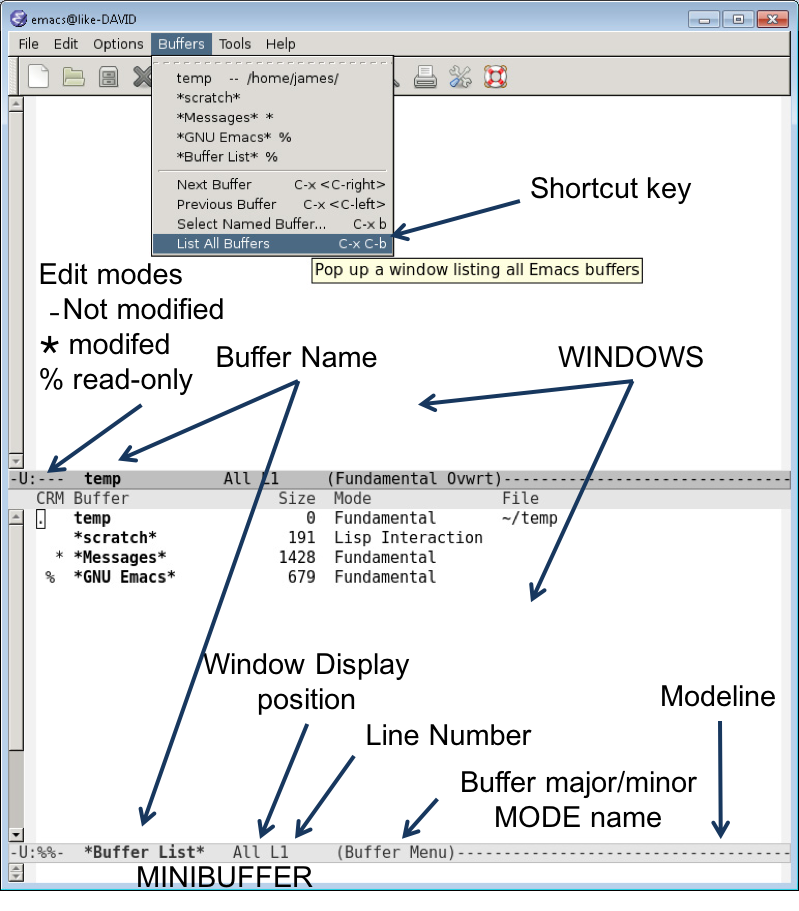
\includegraphics[height=\textheight]{./figure/emacs_layout.png}
\end{figure}
\end{frame}




\begin{frame}[t]{Emacs Preliminaries}
In the emacs documentation, key sequences described as:
\begin{itemize}
\item C-e – This is \keystroke{Ctrl}-\keystroke{e}
\item C-x C-b – This is \keystroke{Ctrl}-\keystroke{x} \keystroke{Ctrl}-\keystroke{b}
\item $\hat{~}$b - this is \keystroke{Ctrl}-\keystroke{b} \
\item C-x b – This is \keystroke{Ctrl}-\keystroke{x} \keystroke{b}
\item M-e – This is \keystroke{Meta}-\keystroke{e} or \keystroke{Alt}-\keystroke{e}
\end{itemize}

\bigskip
On the PC, you can use the \keystroke{Alt} key or \keystroke{Esc}-release to substitute \keystroke{Meta} key

\bigskip
When you press a valid key sequence, emacs executes a command associated with the key
\end{frame}




\begin{frame}[t]{Moving Around}
Emacs uses the control keys to move in the four directions
\bigskip

\keystrokered{Ctrl}-\keystrokered{b} \keystroke{$\leftarrow$} \hfill
\keystrokered{Ctrl}-\keystrokered{n} \keystroke{$\downarrow$} \hfill
\keystrokered{Ctrl}-\keystrokered{p} \keystroke{$\uparrow$} \hfill
\keystrokered{Ctrl}-\keystrokered{f} \keystroke{$\rightarrow$} \hfill



\bigskip
To move by units of word, sentence, and paragraph

\bigskip
\keystrokered{Meta}-\keystrokered{b} Previous word \hfill
\keystrokered{Meta}-\keystrokered{f} Next word \hfill
\keystrokered{Meta}-\keystrokered{a} Previous sentence \hfill
\keystrokered{Meta}-\keystrokered{e} Next sentence \hfill
\keystrokered{Meta}-\keystrokered{\{} Previous paragraph \hfill
\keystrokered{Meta}-\keystrokered{\}} Next paragraph \hfill


\end{frame}



\begin{frame}[t]{Deleting}

Delete a word, line, and sentence
\bigskip

\keystrokered{Ctrl}-\keystrokered{d} Delete a character \hfill
\keystrokered{Meta}-\keystrokered{d} Delete a word \hfill
\keystrokered{Ctrl}-\keystrokered{k} Delete a line \hfill
\keystrokered{Meta}-\keystrokered{k} Delete a sentence \hfill

\bigskip
\begin{block}{When in Doubt}
Use ``\textsc{Get me out of here}'' command \keystrokered{Ctrl}-\keystrokered{g} 
\end{block}
\end{frame}


\begin{frame}[t]{Searching}
\keystroke{Ctrl}-\keystroke{s} asks for searh pattern
\begin{itemize}
\item \keystroke{Ctrl}-\keystroke{s} to search next pattern
\item \keystroke{Ctrl}-\keystroke{r} to search previous pattern
\item Regular expressions can be also used in searching with \keystroke{Meta}-\keystroke{s} 
\end{itemize}

\end{frame}

\begin{frame}[t]{Substitution}
\keystroke{Meta}-\keystroke{$\%$} to replace or \keystroke{Meta}-\texttt{replace-string}
\begin{itemize}
\item Requests for search pattern; press enter for substituting pattern 
\item Replacing the substituting pattern this once \keystroke{SPC}
\item Skipping to the next without replcacing \keystroke{DEL}
\item Replace all remaining matches \keystroke{!}
\item Exiting replace command by \keystroke{RET}
\end{itemize}

\end{frame}


\begin{frame}[t]{Undo and Redo}
Undo an unwanted change is done by \keystroke{Ctrl}-\keystroke{\_}  
\bigskip
Redo is reverse of undo, undo direction is reversed by \keystroke{Ctrl}-\keystroke{g} and \keystroke{Ctrl}-\keystroke{\_}

\end{frame}


\begin{frame}[t]{Macro}
Macros are useful for repeatable key sequences that may be include commands.

\bigskip
Common macro commands
\begin{itemize}
\item \keystroke{Ctrl}-\keystroke{x} - \keystroke{(}– begin macro definition (after this, type whatever actions you would like repeated and stored)       
\item \keystroke{Ctrl}-\keystroke{x} - \keystroke{)}– end macro definition
\item \keystroke{Ctrl}-\keystroke{x} - \keystroke{e} – execute stored macro
\item \keystroke{Ctrl}-\keystroke{u5}  \keystroke{Ctrl}-\keystroke{e} – execute stored macro 5 times (Note: \keystroke{Ctrl}-\keystroke{u5} can prefix any emacs cmd, even a non-cmd)
\end{itemize}
\end{frame}


\begin{frame}[containsverbatim,t]{Simple Tutorial: From Start to quit}
One can type without having to use complex commands but ....
\bigskip
\begin{beamercolorbox}[sep=1em,wd=\linewidth]{boxsthlmLightOrange}
This is how we write \hfill ~~~~~~ \keystroke{Ctrl}-\keystroke{qj} \hfill~~~~~~  and copy lines \hfill ~~~~~~ \keystroke{Ctrl}-\keystroke{p} \hfill~~~~~~  \keystroke{Ctrl}-\keystroke{a}  \hfill~~~~~~   \keystroke{Ctrl}-\keystroke{spc} \hfill~~~~~~    \keystroke{Ctrl}-\keystroke{e} \hfill~~~~~~    \keystroke{Meta}-\keystroke{w} \hfill~~~~~~    \keystroke{Meta}-\keystroke{\}} \hfill~~~~~~    \keystroke{Ctrl}-\keystroke{qj} \hfill~~~~~~    \keystroke{Ctrl}-\keystroke{y} \hfill~~~~~~    \keystroke{Ctrl}-\keystroke{p} \hfill~~~~~~    \keystroke{Ctrl}-\keystroke{a} \hfill~~~~~~    \keystroke{Ctrl}-\keystroke{SPC} \hfill~~~~~~   \keystroke{Ctrl}-\keystroke{u3}  \hfill~~~~~~   \keystroke{Meta}-\keystroke{f} \hfill ~~~~~~   \keystroke{Meta}-\keystroke{w}  \hfill~~~~~~   \keystroke{Meta}-\keystroke{\}}\hfill~~~~~~   \keystroke{SPC} \hfill~~~~~~    \keystroke{Ctrl}-\keystroke{y} \hfill~~~~~~    \keystroke{Return} \hfill~~~~~~   ummm \hfill~~~~~~   \keystroke{Ctrl}-\keystroke{a} \hfill~~~~~~    \keystroke{Ctrl}-\keystroke{u4} \hfill~~~~~~    \keystroke{Ctrl}-\keystroke{d} \hfill~~~~~~   END \hfill~~~~~~   \keystroke{Ctrl}-\keystroke{x-s} ~~~~~~ \keystroke{Ctrl}-\keystroke{x-c}
\end{beamercolorbox}

This will produce following and goes back to command prompt

\begin{beamercolorbox}[wd=\linewidth]{boxsthlmLightPurple}
\begin{sthlmLatex}This is how we write 
and copy lines
This is how we write and copy lines
END\end{sthlmLatex}
\end{beamercolorbox}

\end{frame}



\begin{frame}[containsverbatim,t]{Simple Tutorial: From Start to quit}
\begin{beamercolorbox}[sep=1em,wd=\linewidth]{boxsthlmLightOrange}
{\footnotesize
This is how we write \hfill ~~~~~~ \keystroke{Ctrl}-\keystroke{qj} \hfill~~~~~~  and copy lines \hfill ~~~~~~ \keystroke{Ctrl}-\keystroke{p} \hfill~~~~~~  \keystroke{Ctrl}-\keystroke{a}  \hfill~~~~~~   \keystroke{Ctrl}-\keystroke{spc} \hfill~~~~~~    \keystroke{Ctrl}-\keystroke{e} \hfill~~~~~~    \keystroke{Meta}-\keystroke{w} \hfill~~~~~~    \keystroke{Meta}-\keystroke{\}} \hfill~~~~~~    \keystroke{Ctrl}-\keystroke{qj} \hfill~~~~~~    \keystroke{Ctrl}-\keystroke{y} \hfill~~~~~~    \keystroke{Ctrl}-\keystroke{p} \hfill~~~~~~    \keystroke{Ctrl}-\keystroke{a} \hfill~~~~~~    \keystroke{Ctrl}-\keystroke{SPC} \hfill~~~~~~   \keystroke{Ctrl}-\keystroke{u3}  \hfill~~~~~~   \keystroke{Meta}-\keystroke{f} \hfill ~~~~~~   \keystroke{Meta}-\keystroke{w}  \hfill~~~~~~   \keystroke{Meta}-\keystroke{\}}\hfill~~~~~~   \keystroke{SPC} \hfill~~~~~~    \keystroke{Ctrl}-\keystroke{y} \hfill~~~~~~    \keystroke{Return} \hfill~~~~~~   ummm \hfill~~~~~~   \keystroke{Ctrl}-\keystroke{a} \hfill~~~~~~    \keystroke{Ctrl}-\keystroke{u4} \hfill~~~~~~    \keystroke{Ctrl}-\keystroke{d} ~~~~~~   END ~~~~~~   \keystroke{Ctrl}-\keystroke{x-s} ~~~~~~ \keystroke{Ctrl}-\keystroke{x-c} }
\end{beamercolorbox}

\bigskip
Explaining the commands in the tutorial

\bigskip
{\footnotesize
\keystroke{Ctrl}-\keystroke{qj} Add a new line \hfill
\keystroke{Ctrl}-\keystroke{p} Move to prvious line \hfill
\keystroke{Ctrl}-\keystroke{a} Move to beginning of the sentence \hfill
\keystroke{Ctrl}-\keystroke{spc} Start highlighting \hfill
\keystroke{Ctrl}-\keystroke{e} Move to end of sentence \hfill
\keystroke{Meta}-\keystroke{w} Copy highlighted \hfill
\keystroke{Meta}-\keystroke{\}} Move to end of the paragraph \hfill
\keystroke{Ctrl}-\keystroke{y} Paste copied text \hfill
\keystroke{Ctrl}-\keystroke{u3} Repeat command with following number \hfill
\keystroke{Meta}-\keystroke{f} Move to next word \hfill
\keystroke{Ctrl}-\keystroke{d} Delete a character \hfill
\keystroke{Ctrl}-\keystroke{x-s} Save the document 
\keystroke{Ctrl}-\keystroke{x-c} Quit 
}
\end{frame}



\begin{frame}[containsverbatim,t]{Learn by experience}

\lstinputlisting{./codes/learnbyexperience.txt}


Complete all tasks with minimum number of retyping, but with commands
\begin{itemize}
\item Substitute all j's to z and all z's to j
\item Copy lines 1, 3, 5, and 6, and make new paragraph with those lines
\item Delete three words ``requires extra pluck,'' and type in ``need lot of money'' in the place
\item Add ``caps'' at the end of all words with ``w'', e.g., wizards to ``wizardscaps''
\end{itemize}


\end{frame}


\begin{frame}[t]{References}
Reference card with most commands you’ll ever need
\begin{itemize}
\item \url{http://home.uchicago.edu/~gan/file/emacs.pdf}
\end{itemize}
\bigskip
Official GNU emacs site
\begin{itemize}
\item \url{http://www.gnu.org/software/emacs/}
\end{itemize}

\bigskip
An emacs HowTo
\begin{itemize}
\item \url{https://www.emacswiki.org}
\end{itemize}

\bigskip\centering
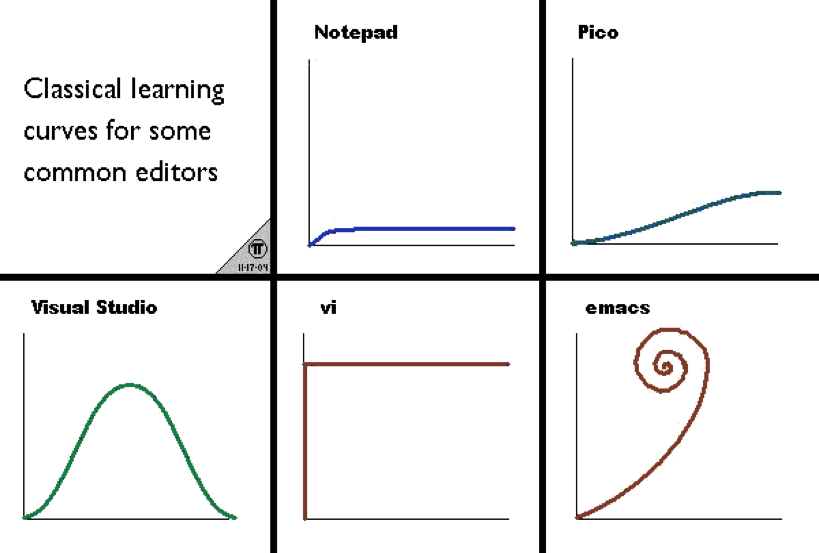
\includegraphics[width=0.5\textwidth]{./figure/learning_curve.png}
\end{frame}





\end{document}
